
\newcommand*{\eg}{e.g.\@\xspace}
\newcommand*{\ie}{i.e.\@\xspace}
\newcommand*{\resp}{resp.\@\xspace}



%%%%%%%%%%%%%%%%%%%%%%%%%%%%%%%%%%%%%%%%%%%%%%%%%%%%%%%%%%%%%%%%%%%%%%%%%%%%%%%%
%%%%%%%%%%%%%%%%%%%%%%%%%%%%%%%% INTRODUCTION %%%%%%%%%%%%%%%%%%%%%%%%%%%%%%%%%%

\section{Introduction}

\begin{figure}
        \begin{subfigure}{0.25\textwidth}
                \centering
                \includegraphics[width=\linewidth]{./figs/trumpet_variations/TpC-ord-G4-mf_withaxes.eps}
                \caption{Trumpet note (\emph{ordinario}).}
                \label{fig:TpC-ord-G4-mf_withaxes}
        \end{subfigure}%
        \begin{subfigure}{0.25\textwidth}
                \centering
                \includegraphics[width=\linewidth]{./figs/trumpet_variations/TpC-ord-G3-mf_withaxes.eps}
                \caption{Pitch (G3).}
                \label{fig:TpC-ord-G3-mf_withaxes}
        \end{subfigure}%

        \begin{subfigure}{0.25\textwidth}
                \centering
                \includegraphics[width=\linewidth]{./figs/trumpet_variations/TpC-ord-G4-pp_withaxes.eps}
                \caption{Intensity (\emph{pianissimo}).}
                \label{fig:TpC-ord-G4-pp_withaxes}
        \end{subfigure}%
        \begin{subfigure}{0.25\textwidth}
                \centering
                \includegraphics[width=\linewidth]{./figs/trumpet_variations/TpC-brassy-G4-ff_withaxes.eps}
                \caption{Tone quality (brassy).}
                \label{fig:TpC-brassy-G4-mf_withaxes}
        \end{subfigure}%

        \begin{subfigure}{0.25\textwidth}
                \centering
                \includegraphics[width=\linewidth]{./figs/trumpet_variations/TpC-sfz-G4-fp_withaxes.eps}
                \caption{Attack (\emph{sfzorzando}).}
                \label{fig:TpC-sfz-G4-fp_withaxes}
        \end{subfigure}%
        \begin{subfigure}{0.25\textwidth}
                \centering
                \includegraphics[width=\linewidth]{./figs/trumpet_variations/TpC-flatt-G4-mf_withaxes.eps}
                \caption{Tonguing (\emph{flatterzunge}).}
                \label{fig:TpC-flatt-G4-mf_withaxes}
        \end{subfigure}


        \begin{subfigure}[b]{0.25\textwidth}
                \centering
                \includegraphics[width=\linewidth]{./figs/trumpet_variations/TpC-trill-maj2-G4-mf_withaxes.eps}
                \caption{Articulation (\emph{trill}).}
                \label{fig:TpC-trill-maj2-G4-mf_withaxes}
        \end{subfigure}%
        \begin{subfigure}[b]{0.25\textwidth}
                \centering
                \includegraphics[width=\linewidth]{./figs/trumpet_variations/TpC+H-ord-G4-mf_withaxes.eps}
                \caption{Mute (\emph{harmon}).}
                \label{fig:TpC+H-ord-G4-mf_withaxes}
        \end{subfigure}

        \begin{subfigure}[b]{0.25\textwidth}
                \centering
                \includegraphics[width=\linewidth]{./figs/trumpet_variations/TpC-voc-harms-C4-mf_withaxes.eps}
                \caption{Phrasing (\emph{d\'{e}tach\'{e}}).}
                \label{fig:TpC+voc-harms-G4-mf_withaxes}
        \end{subfigure}%
        \begin{subfigure}[b]{0.25\textwidth}
                \centering
                \includegraphics[width=\linewidth]{./figs/trumpet_variations/Vn-ord-G4-mf-4c_withaxes.eps}
                \caption{Instrument (violin).}
                \label{fig:Vn-ord-G4-mf-4c}
        \end{subfigure}
        \caption{Ten factors of variations of a musical note.}\label{fig:trumpet-variations}
\end{figure}

The gradual diversification of the timbral palette in Western classical music at the turn of the 20th century is reflected in five concurrent trends:
the addition of new instruments to the symphonic instrumentarium, either by technological inventions (\eg theremin) or importation from non-Western musical cultures (\eg marimba) \cite[epilogue]{sachs2012book};
the creation of novel instrumental associations, as epitomized by \emph{Klangfarbenmelodie} \cite[chapter 22]{schoenberg2010book};
the temporary alteration of resonant properties through mutes and other ``preparations'' \cite{dianova2007phd};
a more systematic usage of extended instrumental techniques, such as artificial harmonics, \emph{col legno batutto}, or flutter tonguing \cite[chapter 11]{kostka2016book};
and the resort to electronics and digital audio effects \cite{zolzer2011dafx}.
The first of these trends has somewhat stalled: to this day, most Western composers rely on an acoustic instrumentarium that is only marginally different from the one that was available in the Late Romantic period.
Nevertheless, the latter approaches to timbral diversification were massively adopted into post-war contemporary music.
In particular, an increased concern for the concept of musical gesture \cite{godoy2009book} has liberated many unconventional instrumental techniques from their figurativistic connotations, thus making the so-called ``ordinary'' playing style merely one of many compositional -- and improvisational -- options.

Far from being exclusive to erudite music, extended playing techniques are also commonly found in oral tradition; in some cases, they even stand out as a distinctive component of musical style.
Four well-known examples are:
the snap pizzicato (``slap'') of the upright bass in rockabilly,
the growl of the tenor saxophone in rock'n'roll,
the shuffle stroke of the violin (``fiddle'') in Irish folklore,
and the glissando of the clarinet in Klezmer music.
Consequently, the mere knowledge of organology (the instrumental \emph{what?}~of music), as opposed to chironomics (its gestural \emph{how?}), is a rather weak source of information for browsing and recommendation in large music databases.

Yet, past research in music information retrieval (MIR), and especially machine listening, rarely acknowledges the benefits of integrating the influence of performer gestures into a coherent taxonomy of musical instrument sounds.
Instead, gestures are either framed as a spurious form of intra-class variability between instruments, without delving into its interdependencies with pitch and intensity;
or, symmetrically, as a probe for the acoustical study of a given instrument, without enough emphasis onto the broader picture of orchestral diversity.

One major cause of this gap in research is the difficulty of collecting and annotating data for contemporary instrumental techniques.
Fortunately, such obstacle has recently been overcome, owing to the creation of databases of instrumental samples in a perspective of spectralist music orchestration \cite{maresz2013cmr}.
In this article, we capitalize on the availability of data to formulate a new line of research in MIR, namely the joint retrieval of organological information (``\emph{what} instrument is being played in this recording?'') and chironomical information (``\emph{how} is the musician producing sound?''), while remaining invariant to other factors of variability, which are deliberately regarded as contextual: at what pitches and intensities, but also where, when, why, by whom, and for whom was the music recorded.

Figure \ref{fig:TpC-ord-G4-mf_withaxes} shows the constant-$Q$ wavelet scalogram (\ie{} the complex modulus of the constant-$Q$ wavelet transform) of a trumpet musical note, as played with an ordinary technique.
Unlike most existing publications on instrument classification, which exclusively focus on pitch (Figure \ref{fig:TpC-ord-G3-mf_withaxes}) and intensity (Figure \ref{fig:TpC-ord-G4-pp_withaxes}) as the main factors of intra-class variability, this paper aims at accounting for the presence of instrumental playing techniques (IPT), such as changes in tone quality (Figure \ref{fig:TpC-brassy-G4-mf_withaxes}), attack (Figure \ref{fig:TpC-sfz-G4-fp_withaxes}), tonguing (Figure \ref{fig:TpC-flatt-G4-mf_withaxes}), and articulation (Figure \ref{fig:TpC+H-ord-G4-mf_withaxes}), either as intra-class variability (instrument recognition task) or as inter-class variability (IPT recognition task).
The analysis of IPTs whose definition necessarily involves more than a single musical event, such as phrasing (Figure \ref{fig:TpC+voc-harms-G4-mf_withaxes}), is beyond the scope of this paper.

Section 2 reviews the existing literature on the topic.
Section 3 derives the task of IPT classification from the definition of both a taxonomy of instruments and a taxonomy of gestures.
Section 4 describes how two topics in machine listening, namely scattering transforms and supervised metric learning, are relevant to address this task.
Section 5 reports the results from an IPT classification benchmark on the Studio On Line (SOL) dataset.



%%%%%%%%%%%%%%%%%%%%%%%%%%%%%%%%%%%%%%%%%%%%%%%%%%%%%%%%%%%%%%%%%%%%%%%%%%%%%%%%
%%%%%%%%%%%%%%%%%%%%%%%%%%%%%%%%  RELATED WORK  %%%%%%%%%%%%%%%%%%%%%%%%%%%%%%%%
\section{Related work}
This section reviews some of the recent MIR literature on the audio analysis of instrumental playing techniques,
with a focus on the available datasets for each formulation of the problem at hand.

\subsection{Classification of ordinary isolated notes}
The earliest works on musical instrument recognition restricted their scope to individual notes played with an ordinary technique -- with datasets such as MUMS \cite{opolko1989dataset}, MIS, RWC \cite{goto2003ismir}, and Philharmonia -- thus eliminating most factors of intra-class variability due to the performer  \cite{martin1998asa,brown1999jasa,eronen2000icassp,herrera2003jnmr,wieczorkowska2003jiis,kaminskyj2005jiis,benetos2006icassp}.
These works have culminated with the development of a support vector machine (SVM) classifier trained on spectrotemporal receptive fields (STRF), which are idealized computational models of neurophysiological responses in the central auditory system \cite{chi2005jasa}.
Not only did it attain a near-perfect mean accuracy of $98.7\%$ on the RWC dataset, but the confusion matrix of its automated predictions was closely similar to the confusion matrix of human listeners \cite{patil2012plos}.
Therefore, the supervised classification of musical instruments from recordings of ordinary notes could arguably be considered a solved problem; we refer to \cite{bhalke2016jiis} for a recent review of the state of the art.

\subsection{Classification of solo recordings}
One straightforward extension of the problem above is the classification of solo phrases, encompassing some variability in melody \cite{krishna2004icassp}, for which the accuracy of STRF models is around $80\%$ \cite{patil2015eurasip}.
Since the Western tradition of solo music is essentially limited to a narrow range of instruments (\eg{} piano, classical guitar, violin) and genres (sonatas, contemporary, free jazz, folk), datasets of solo phrases, such as solosDb \cite{joder2009taslp}, are exposed to strong biases.
This issue is partially mitigated by the recent surge of multitrack datasets, such as MedleyDB \cite{bittner2014ismir}, which has spurred a renewed interest in single-label instrument classification \cite{yip2017ismir}.
In addition, the cross-collection evaluation methodology \cite{livshin2003ismir} allows to prevent the risk of overfitting caused by the relative homogeneity of these small datasets in terms of artists and recording conditions \cite{bogdanov2016ismir}.
To this date, the best classifier of solo recordings is a spiral convolutional network \cite{lostanlen2016ismir} trained on the Medley-solos-DB dataset \cite{lostanlen2018msdb}, \ie{} a cross-collection dataset which aggregates MedleyDB and solosDb following the procedure of \cite{donnelly2015icdmw}.
We refer to \cite{han2017taslp} for a recent review of the state of the art.

\subsection{Multilabel classification in polyphonic mixtures}
Because most publicly released musical recordings are polyphonic, the generic formulation of instrument recognition as a multilabel classification task is the most appropriate for large-scale deployment \cite{martins2007ismir,burred2009icassp}.
However, it suffers from two methodological caveats: first, polyphonic instrumentation is not independent from other attributes of information, such as geographical origin, genre, or key; and secondly, the inter-rater agreement decreases with the number of overlapping sources \cite[chapter 6]{fuhrmann2012phd}.
Such issues are all the more troublesome that there is, to this date, no  annotated dataset of polyphonic mixtures that is diverse enough to be devoid of artist bias.
The Open-MIC initiative, from the newly created Community for Open and Sustainable Music and Information Research (COSMIR), might contribute to mitigating them in the near future \cite{mcfee2016ismir}.

\subsection{Single-instrument playing technique classification}
Lastly, there is a growing interest for studying the role of the performer in musical acoustics, from both perspectives of sound production and sound perception.
Besides its interest in audio signal processing, this topic is connected to other disciplines, such as biomechanics and gestural interfaces \cite{metcalf2014frontiers}.
The majority of the available literature focuses on the range of IPTs afforded by a single instrument: recent examples include clarinet \cite{loureiro2004ismir}, percussion \cite{tindale2004ismir}, piano \cite{bernays2013smc}, guitar \cite{foulon2013cmmr,su2014ismir,chen2015ismir}, violin \cite{young2008nime}, cello \cite[chapter 6]{chudy2016phd}, and erhu \cite{yang2014fma}.
Some publications frame timbral similarity in a polyphonic setting, yet do so according to a purely perceptual definition of timbre -- with continuous attributes such as brightness, warmth, dullness, roughness, and so forth -- without connecting these attributes to the discrete latent space of IPTs \cite{antoine2018isma}.

In this paper, we formulate the retrieval of expressive parameters of musical timbre at the scale of the symphonic orchestra at large, while expliciting these parameters in terms of sound production (\ie{} through a finite set of instructions, readily interpretable by the performer) rather than by means of perceptual epithets only.
We refer to \cite{leman2017chapter} for a recent review of the state of the art.



%%%%%%%%%%%%%%%%%%%%%%%%%%%%%%%%%%%%%%%%%%%%%%%%%%%%%%%%%%%%%%%%%%%%%%%%%%%%%%%%
%%%%%%%%%%%%%%%%%%%%%%%%%%%%%%%%%%%  TASKS  %%%%%%%%%%%%%%%%%%%%%%%%%%%%%%%%%%%%
\section{Tasks}
In this section, we distinguish taxonomies of musical instruments from taxonomies of musical gestures.

\subsection{Taxonomies}

The Hornbostel-Sachs taxonomy (H-S) strives to organize the diversity of musical instruments according to their manufactural characteristics only, and is purposefully unaffected by sociohistorical background \cite{montagu2009muzyka}.
Because it offers an unequivocal way of describing any acoustic instrument without any prior knowledge on its applicable IPTs, it serves as a \emph{lingua franca} in ethnomusicology and museology, especially for ancient or rare instruments which may lack available informants.
The location of the violin in H-S (321.321-71), as depicted in Figure \ref{fig:instrument-dendrogram}, also encompasses the viola and the cello in addition to the violin.
This is because these three instruments, viewed as inert objects, share a common morphology, despite differences in posture for the performer: both violin and viola are usually played under the jaw whereas the cello is held between the knees.
Accounting for these differences begs to refine H-S by means a vernacular taxonomy.
Most instrument taxonomies in music signal processing, including MedleyDB and AudioSet \cite{gemmeke2017icassp}, reach the vernacular level rather than conflating all instruments belonging to the same H-S node.
In some cases, an even finer level of granularity is attained by the listing of potential alterations to the instrument -- be them permanent or temporary, at the time scale of more than a single note -- that affect its resonant properties after the end of the conventional manufacturing process, \eg{} mutes and other preparations \cite{dianova2007phd}.
The only example of node in the MedleyDB taxonomy reaching this level is \emph{tack piano} \cite{bittner2014ismir} .

\begin{figure}[t!]
\centering
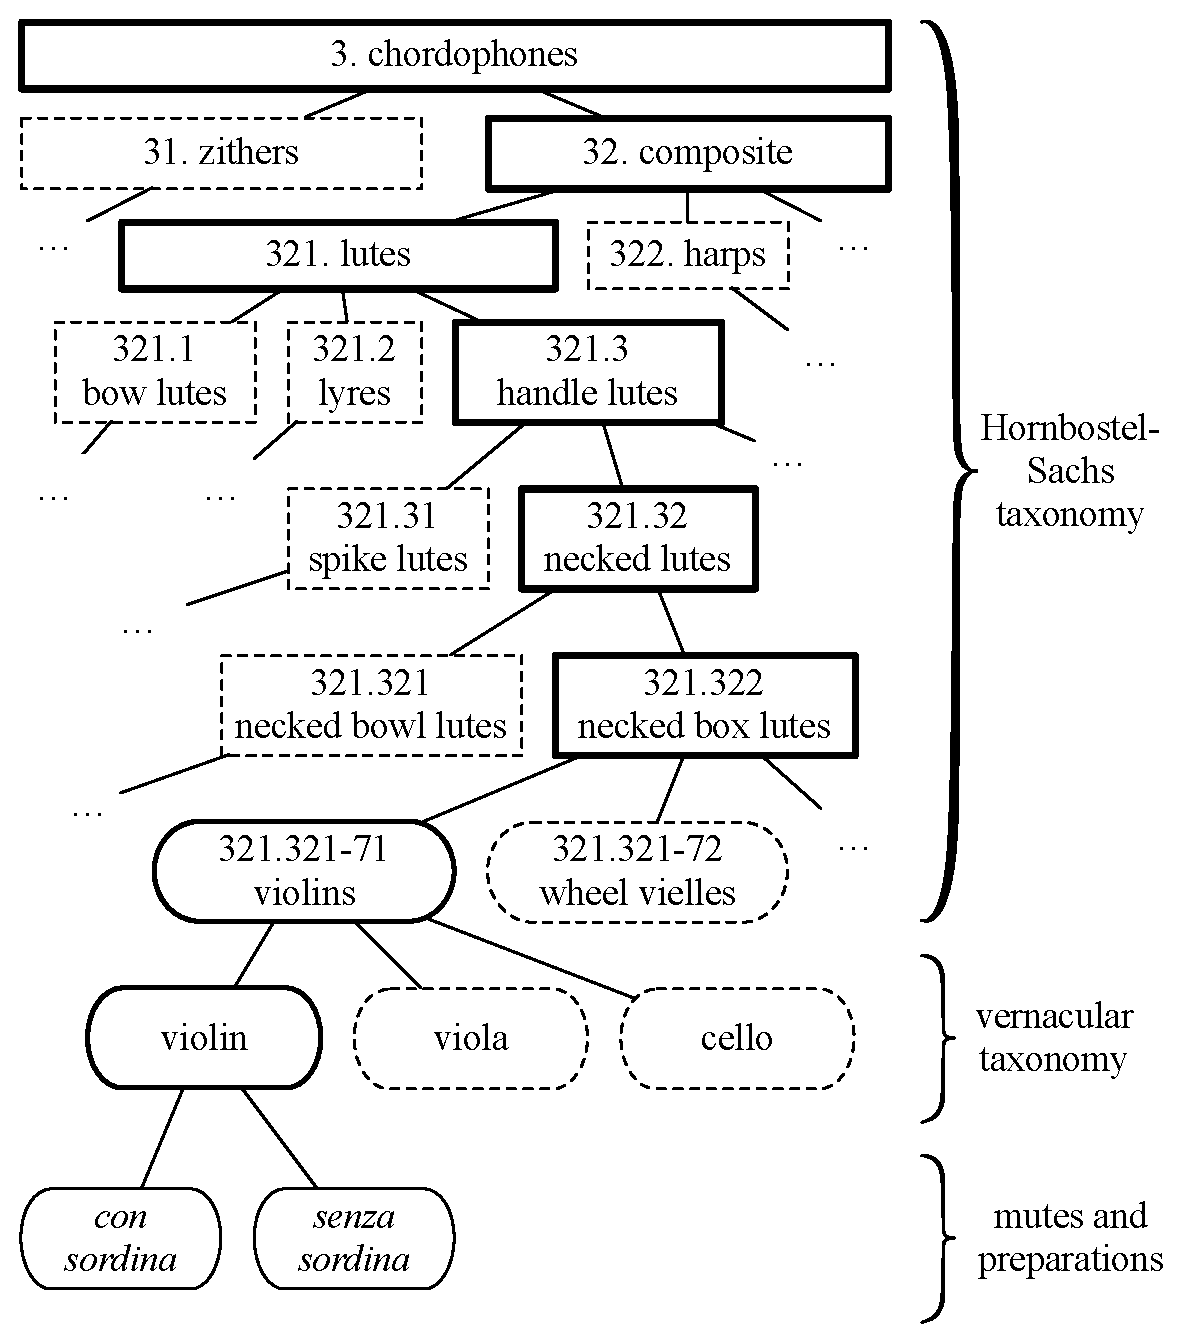
\includegraphics[width=\linewidth]{./figs/dendrograms/instrument-dendrogram.eps}
\caption{Taxonomy of musical instruments.}
\label{fig:instrument-dendrogram}
\end{figure}

Unlike musical instruments, which are approximately amenable to a hierarchical taxonomy of resonating objects, IPTs result from a complex synchronization between multiple gestures, which may involve both hands and arms, as well as diaphragm, vocal tract, and sometimes the whole body.
As a result, there is no immediate way to interface them with H-S, or indeed any tree-like structure \cite{kolozali2011ismir}.
Instead, every playing technique is described by a finite collection of categories, each belonging to a different ``name\-space''; Figure \ref{fig:technique-dendrogram} illustrates such namespaces in the case of the violin.
It therefore appears that, rather than aiming for a mere increase in granularity with respect to H-S, a coherent research program around extended playing techniques should formulate them as belonging to a meronomy, \ie{} a modular entanglement of part-whole relationships, in the fashion of the Visipedia initiative in computer vision \cite{belongie2015pattern}.
In recent years, some publications have attempted to lay the foundations of such a modular approach, with the aim of making H-S relevant to contemporary music creation \cite{magnusson2017jnmr,weisser2011ytm}; yet, such considerations are still in large part speculative, and offer no definitive procedure for evaluating, let alone training, information retrieval systems.

\begin{figure}
\centering
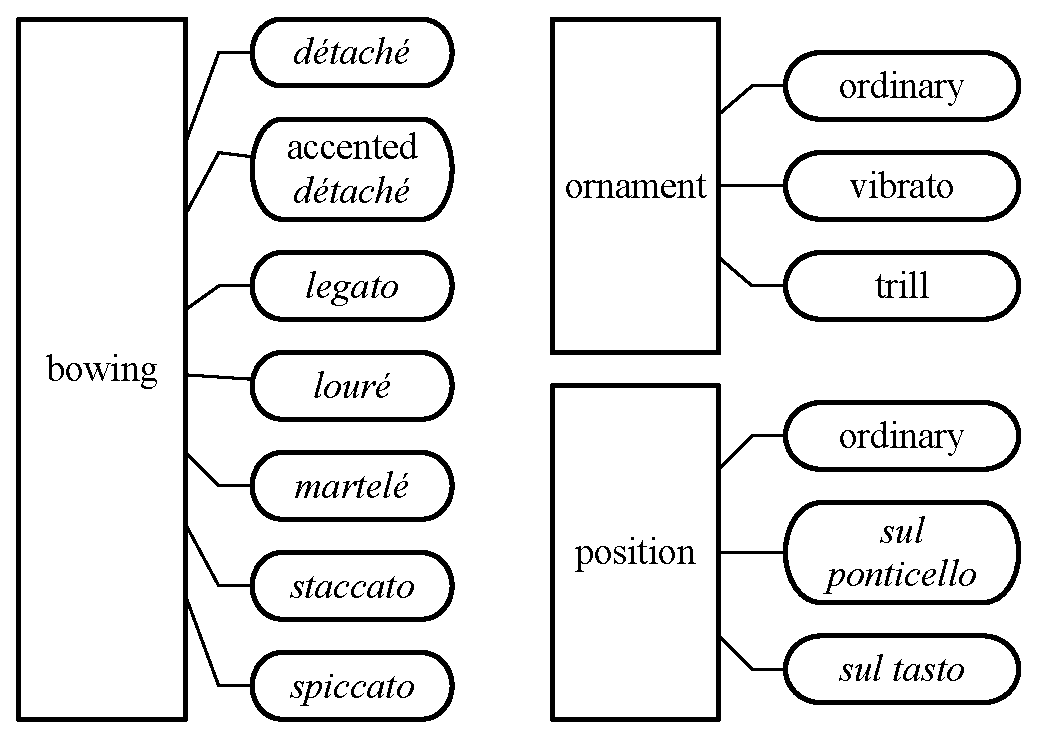
\includegraphics[width=\linewidth]{./figs/dendrograms/technique-dendrogram.eps}
\caption{Namespaces of violin playing techniques.}
\label{fig:technique-dendrogram}
\end{figure}


\subsection{Application setting and evaluation} \label{sec:motivation}

In what follows, we adopt a middle ground position between the two aforementioned approaches: neither a supervised classifier (as in a hierarchical taxonomy), nor a caption generator (as in a meronomy), our system is a query-by-example search engine in a large database of isolated notes.
This system is meant to provide a small number $k$ of nearest neighbors in the dataset of musical instrument samples to any user-defined audio query $\boldsymbol{x}(t)$.
In the context of contemporary music creation, this $\boldsymbol{x}(t)$ may be an instrumental or vocal sketch; a sound event recorded from the environment; a computer-generated waveform; or any mixture of the above \cite{maresz2013cmr}.
Upon inspecting the $k$ nearest neighbors returned by the search engine, the composer may decide to retain one of the retrieved notes, in which case its attributes (pitch and intensity, but also the exact playing technique) are readily available and can be included into the musical score to approximate the query.

Faithfully evaluating such a system is a difficult procedure, and ultimately would rest on its practical usability, as judged by the composers themselves.
Nevertheless, a useful quantitative metric for this task is the precision at $k$ (P@$k$) of the test set with respect to the training set, both under a instrument taxonomy and an IPT taxonomy.
In all subsequent experiments, we report $P@k$ after setting the number of retrieved items to $k=5$.

\subsection{Studio On Line dataset (SOL)}

The Studio On Line dataset (SOL) was recorded at Ircam in 2002 and is freely downloadable as part of the Orchids software for computer-assisted orchestration.\footnote{Link to SOL dataset: \url{http://forumnet.ircam.fr/product/orchids-en/}}
It comprises 16 musical instruments playing $25444$ isolated notes in total.
The distribution of these notes, shown in Figure \ref{fig:instrument-histogram}, spans the full combinatorial diversity of applicable intensities, pitches, preparations (\ie{} mutes), as well as all applicable playing techniques.
The distribution of playing techniques -- whose most common are shown in Figure \ref{fig:technique-histogram} -- is heavy-tailed (average $178$, standard deviation $429$): this is because some playing techniques are shared between many instruments (\eg{} \textit{tremolo}) whereas other are instrument-specific (\eg{} \textit{xylophonic} which is specific to the harp).
The SOL dataset has $143$ IPTs in total, and $469$ applicable instrument-mute-technique triplets.

\begin{figure}[t!]
\centering
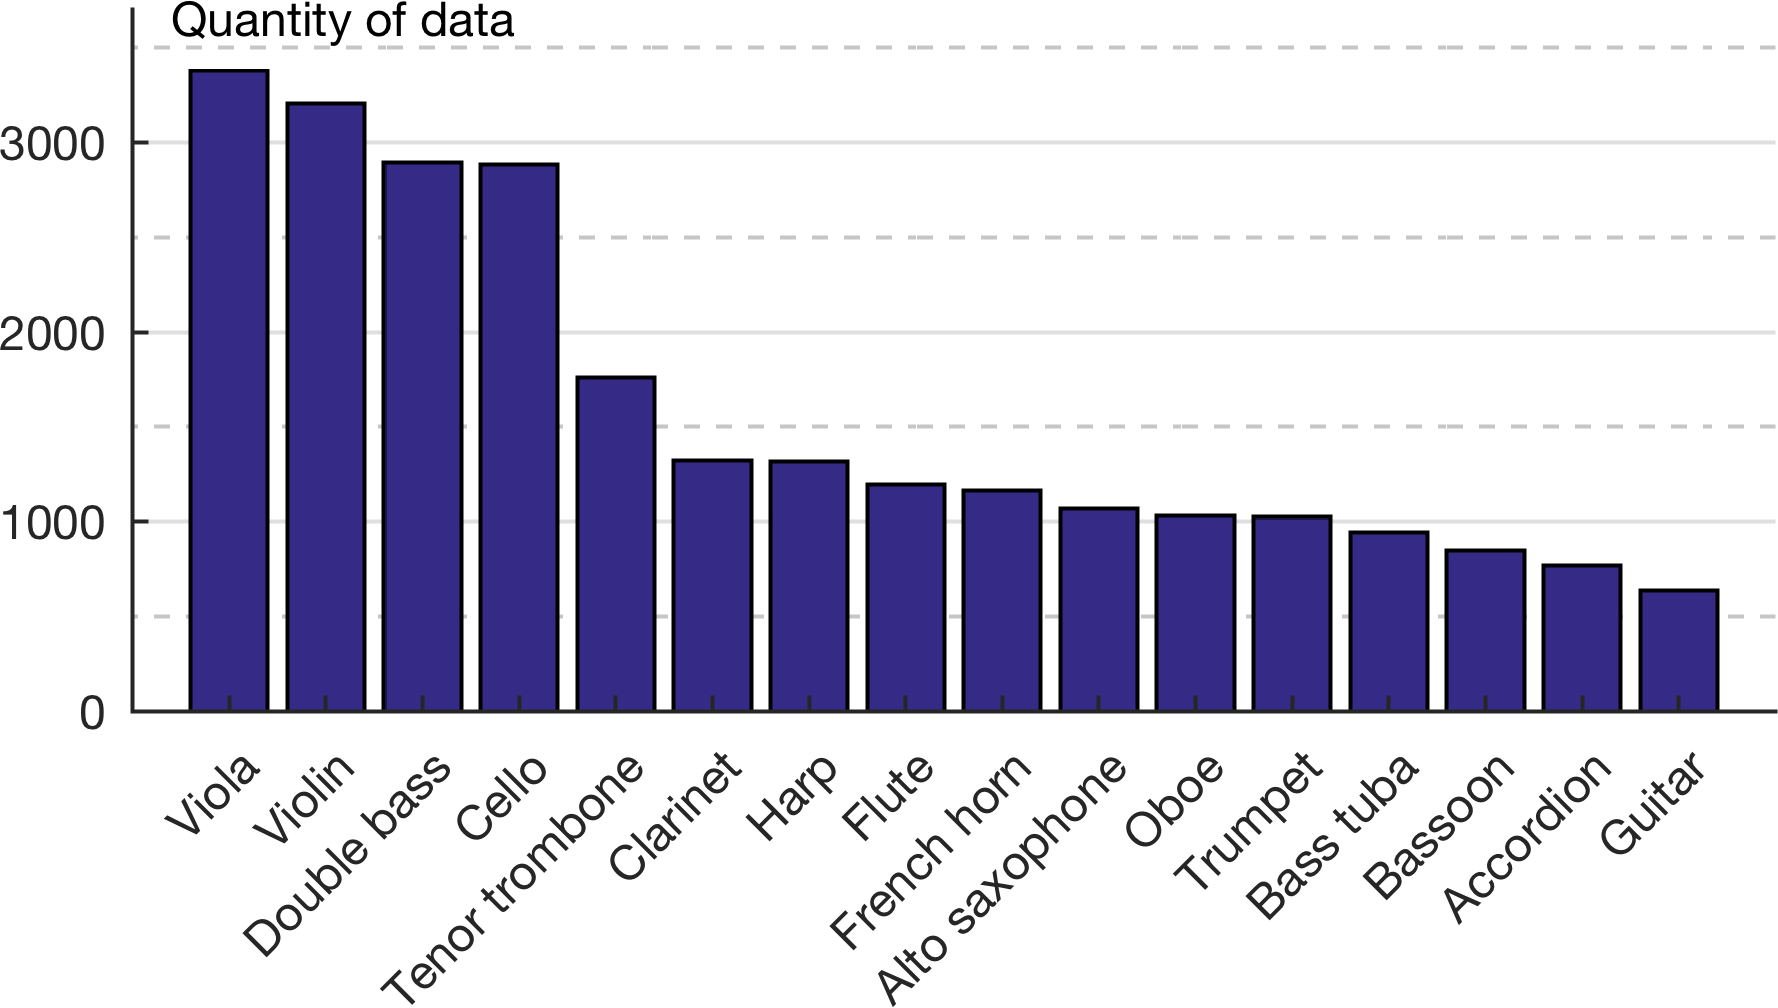
\includegraphics[width=\linewidth]{./figs/histogram/histogram_instruments.png}
\caption{Instruments in the SOL dataset.}
\label{fig:instrument-histogram}
\end{figure}

\begin{figure}[h!]
\centering
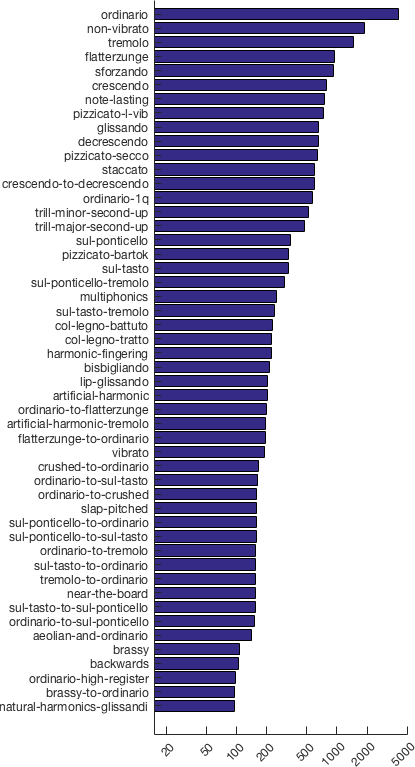
\includegraphics[width=\linewidth]{./figs/histogram/histogram_modes.png}
\caption{Playing techniques in the SOL dataset.}
\label{fig:technique-histogram}
\end{figure}


% Bows and mallets are part of the gesture
% The use of mutes is part of the instrument BUT any gesture while holding the mute (e.g.  trombone) creates a new IPT category that is distinct from ordinary style.

% Out of scope are:
% Variations in articulation: trill, slide. Unlike vibrato, they have a melodic function.
% Variations in: artificial harmonics, subharmonics [ref Mari Kimura],
% Variations in phrasing: arpeggio,
% analog FX



%%%%%%%%%%%%%%%%%%%%%%%%%%%%%%%%%%%%%%%%%%%%%%%%%%%%%%%%%%%%%%%%%%%%%%%%%%%%%%%%
%%%%%%%%%%%%%%%%%%%%%%%%%%%%% ACKNOWLEDGMENTS %%%%%%%%%%%%%%%%%%%%%%%%%%%%%%%%%%

\begin{acks}
The authors wish to thank Philippe Brandeis for fruitful discussions on contemporary music creation
%, Andrew Farnsworth and Grant Van Horn for fruitful discussions on Visipedia,
and Katherine Crocker for helpful suggestions on the title of this article.
\end{acks}
